\documentclass[border=10pt]{standalone}
\usepackage[svgnames]{xcolor}
\usepackage{amsmath}
\usepackage{pgfplots}
\pgfplotsset{compat=newest}
\usepackage[sfdefault]{FiraSans}
\usepackage{FiraMono}
\renewcommand*\familydefault{\sfdefault}
\begin{document}
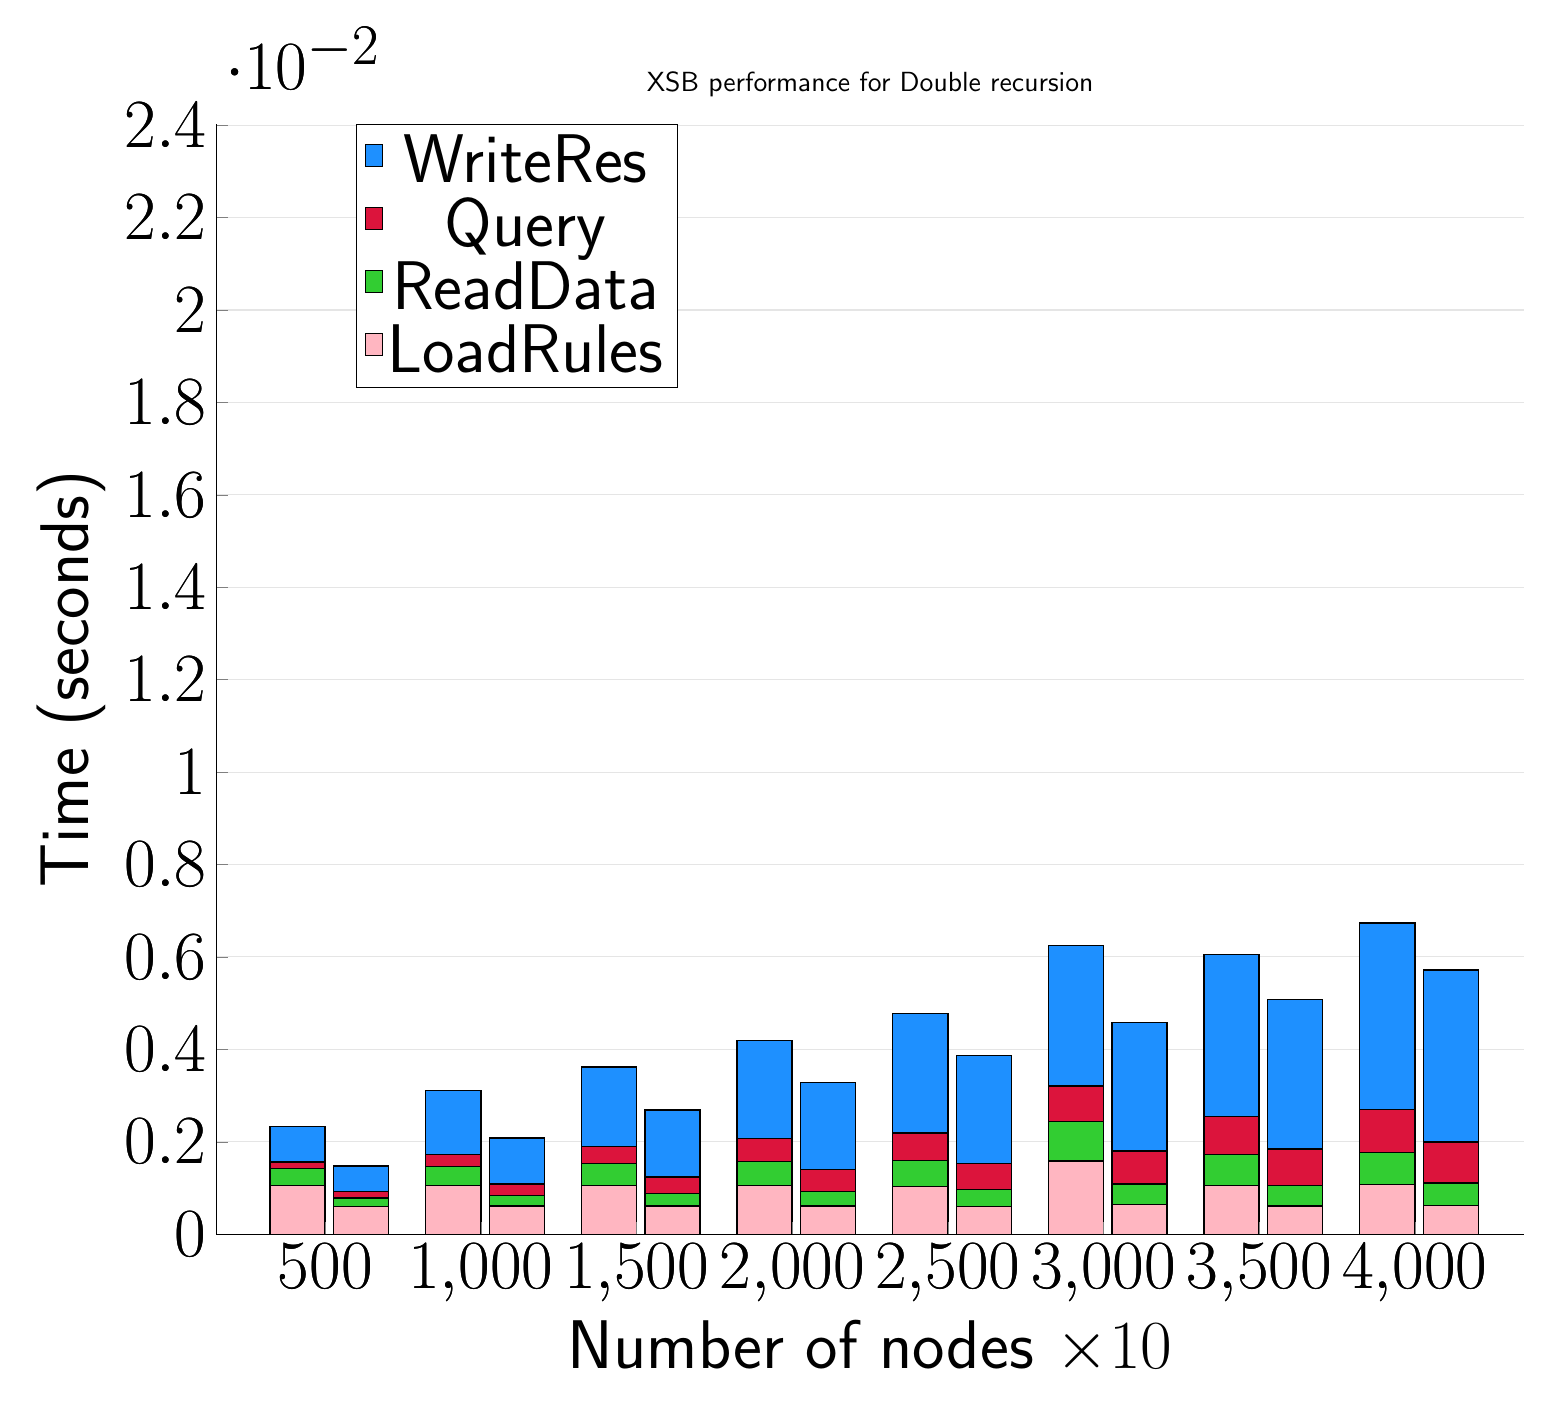
\begin{tikzpicture}
\begin{axis}[
   ybar stacked,
   title={XSB performance for Double recursion},
   bar shift=-10pt,
   width=1.5\textwidth,
   bar width=0.7cm,
   ymajorgrids, tick align=inside,
   major grid style={draw=gray!20},
   xtick=data,
   ymin=0, ymax=0.024034543037414553,
   axis x line*=bottom,
   axis y line*=left,
   enlarge x limits=0.1,
   legend style={
       at={(0.23, 1)},
       anchor=north,
       legend columns=1,
       font=\Huge,
   },
   ylabel={Time (seconds)},
   xlabel={Number of nodes $\times 10$},
   label style={font=\Huge},
   tick label style={font=\Huge},
]
\addlegendimage{fill=DodgerBlue, draw=black, line width=0.2pt}
\addlegendentry{WriteRes}
\addlegendimage{fill=Crimson, draw=black, line width=0.2pt}
\addlegendentry{Query}
\addlegendimage{fill=LimeGreen, draw=black, line width=0.2pt}
\addlegendentry{ReadData}
\addlegendimage{fill=LightPink, draw=black, line width=0.2pt}
\addlegendentry{LoadRules}
\addplot +[fill=LightPink, draw=black, line width=0.5pt] coordinates {
    (500, 0.0010525703430175777)
    (1000, 0.001058602333068848)
    (1500, 0.001050996780395508)
    (2000, 0.001051306724548341)
    (2500, 0.001033115386962891)
    (3000, 0.001585125923156739)
    (3500, 0.0010538816452026361)
    (4000, 0.001071357727050783)
};
\addplot +[fill=LimeGreen, draw=black, line width=0.5pt] coordinates {
    (500, 0.0003638029098510741)
    (1000, 0.00040769577026367177)
    (1500, 0.00048105716705322267)
    (2000, 0.0005259990692138671)
    (2500, 0.0005658149719238281)
    (3000, 0.0008583784103393551)
    (3500, 0.0006737947463989258)
    (4000, 0.00070340633392334)
};
\addplot +[fill=Crimson, draw=black, line width=0.5pt] coordinates {
    (500, 0.00014543533325195307)
    (1000, 0.0002584934234619142)
    (1500, 0.00036983489990234387)
    (2000, 0.0005003929138183595)
    (2500, 0.00058746337890625)
    (3000, 0.0007629156112670902)
    (3500, 0.000815129280090332)
    (4000, 0.000926852226257324)
};
\addplot +[fill=DodgerBlue, draw=black, line width=0.5pt] coordinates {
    (500, 0.0007720947265625)
    (1000, 0.0013885498046874996)
    (1500, 0.0017130136489868163)
    (2000, 0.0021108150482177734)
    (2500, 0.002595257759094238)
    (3000, 0.0030437231063842767)
    (3500, 0.0035124063491821303)
    (4000, 0.004034543037414551)
};
\end{axis}
\begin{axis}[
   ybar stacked,
   bar shift=13pt,
   width=1.5\textwidth,
   bar width=0.7cm,
   ymajorgrids, tick align=inside,
   major grid style={draw=none},
   xtick=data,
   ymin=0, ymax=0.024034543037414553,
   axis x line*=none,
   axis y line*=none,
   enlarge x limits=0.1,
   label style={font=\Huge},
   tick label style={font=\Huge},
]
\addplot +[fill=LightPink, draw=black, line width=0.5pt] coordinates {
    (500, 0.0006041000000000001)
    (1000, 0.0006102)
    (1500, 0.0006064999999999999)
    (2000, 0.0006098000000000001)
    (2500, 0.0006052000000000005)
    (3000, 0.0006446000000000001)
    (3500, 0.0006081999999999997)
    (4000, 0.0006175999999999996)
};
\addplot +[fill=LimeGreen, draw=black, line width=0.5pt] coordinates {
    (500, 0.0001790999999999999)
    (1000, 0.0002257999999999998)
    (1500, 0.0002743999999999998)
    (2000, 0.00031769999999999943)
    (2500, 0.00035899999999999984)
    (3000, 0.0004380999999999997)
    (3500, 0.00044720000000000014)
    (4000, 0.0004875)
};
\addplot +[fill=Crimson, draw=black, line width=0.5pt] coordinates {
    (500, 0.0001370999999999997)
    (1000, 0.00024749999999999984)
    (1500, 0.00035420000000000037)
    (2000, 0.0004729000000000006)
    (2500, 0.0005638)
    (3000, 0.0007155)
    (3500, 0.0007889000000000001)
    (4000, 0.0008934999999999997)
};
\addplot +[fill=DodgerBlue, draw=black, line width=0.5pt] coordinates {
    (500, 0.0005575000000000004)
    (1000, 0.0010021000000000003)
    (1500, 0.0014492999999999997)
    (2000, 0.0018818999999999995)
    (2500, 0.0023456)
    (3000, 0.0027854999999999998)
    (3500, 0.0032363)
    (4000, 0.003717900000000001)
};
\end{axis}
\end{tikzpicture}

\end{document}
